\chapter{Introduction}

The non-linear behavior of superconducting nanowires is a crucial aspect of many of their applications, including superconducting nanowire single-photon detectors (SNSPDs) and neuromorphic computing \cite{snspd_original_paper, spiking_nn}. However, this non-linearity also makes it challenging to simulate nanowires, particularly when considering their microwave properties. One common method of simulating these nanowire electronics relies on existing circuit simulation environments \cite{karl_spice}. These environments were optimized for classical electronics and lack optimizations that account for the microwave and superconducting characteristics of the models.

While plenty of good superconducting simulators exist for the frequency domain
modeling of devices, they tend to neglect effects that nanowire-based device 
designer care about \cite{josephsoncircsjl, wrspice}. These effects include simulating pulses, thermal modeling
of hotspot generation, and thermal coupling in stacks.
Simulating the dominant effects in our superconducting electronics in the time domain
is a crucial step for device design.

As we scale device sizes and introduce dependence on thermal effects and electrostatic coupling, the complexity of the models makes it increasingly difficult to accurately and efficiently simulate the device's time behavior properly.
While the need for more accurate nanowire simulations and the complexity of our models continue to grow, the tools used to simulate these devices must also evolve to meet these challenges. We aim to address that
by introducing wrappers around existing SPICE software, a method for quickly
assessing simulation stability and present the building blocks for a new
nanowire electronics simulator built in Julia.

\section{Non-linearity in superconducting nanowires}\label{nonlinearity}

Superconducting nanowires are highly non-linear and present three main forms of non-linearity:
(1) kinetic inductance, (2) normal-superconducting state transitions and
(3) coupling to other non-linear dynamics.

Kinetic inductance in superconducting nanowires is a continuous form of non-linearity introduced by the 
cooper pair dependence on the bias current in a nanowire \cite{inductance_nonlinearity}. In thin films, kinetic inductance is highly dependent on the film thickness
and temperature \cite{dizhu-thesis}. 
A nanowire's inductance is almost entirely due to kinetic inductance, and therefore
its reliance on the bias current is of importance \cite{kinetic_inductance_majority_of_nw}.
Designing more complicated electronics and SNSPDs  requires
us to simulate the effects of current behavior other than DC (such as pulses)
on the kinetic inductance. This effect is important as 
the non-linearity of the nanowire can change the shapes of pulses -- this is a well-studied effect in non-linear transmission lines \cite{nl_tline_reshape}. 
Accounting for the non-linear microwave properties causes even simple designs 
-- such as a superconducting transmission line operating only in the superconducting regime -- to 
behave in a difficult-to-anticipate non-linear fashion. 

The second form of non-linearity pertains to the superconducting state. By assuming the device is
experiencing a constant temperature, there is a constant threshold critical current
$i_c$ where if the current exceeds $i_c$ locally along a nanowire, it switches into the resistive state. This switching behavior is a non-linearity
over a Boolean state that is dependent on the current flowing through each portion of the nanowire.
Nonlinearities over a Boolean state are particularly hard to simulate as they involve sudden large
magnitude changes. Typical non-linear solvers are optimized for continuous non-linear systems where
the solver enters a loop making the time step smaller until the magnitude of change is small \cite{spice-book, hspice}.
In Boolean states, there is no sense of continuity, and in the limit of smaller time steps, the 
change in response magnitude will be just as large. 

\section{Nanowire Elements}

From an electronics standpoint, a nanowire's lumped model is a non-linear inductor when superconducting. When resistive, an additional resistor is in series with that inductor.
These two building blocks (a continuously non-linear inductor and a discrete non-linear
resistance) are the basis for modeling the behavior of superconducting nanowires in
the electronics picture. This model covers the two main types of nonlinearities
exhibited by nanowires.

A more complicated - but sometimes necessary - picture includes coupling to a thermal equation.
A nanowire's critical current $i_c$ and critical temperature $T_c$ are
functions of the current state of the superconductor. These two parameters are related by the critical
surface; leading to implications such as $T_c(i=0) \neq T_c(i=0.75i_c)$. 
The superconducting-to-normal state transition
begins a coupled chain reaction between a thermal system and an electrical system, making
modeling nanowires harder. When a portion of the nanowire switches into the resistive 
state, a normal region starts to form in the wire that dissipates thermal energy. This
energy heats up the surrounding portions of the nanowire, decreasing their critical 
current. At the same time, the normal region has a higher impedance than the nanowire
diverting current around it, allowing portions of the nanowire to see a higher density of
the current, making it more likely to switch in the plane of the hotspot. The hotspot also
dissipates heat to the stack and fridge. These are well-studied phenomena for nanowires
and tend to be modeled through experimentally fitted parameters \cite{phen_model, karl_spice}. \todoexplain[]{maybe talk about simulating noise transition??}

Another picture that tends to be neglected is the distributed picture of the nanowire.
In reality, the nanowire has a spatial dimension to it and is a microwave device
\cite{distributed_nanowire_model, santavicca_microwave}. This
picture tends to enforce simulation constraints as the discretization and network size
increase. This picture accounts for time delays introduced to a signal entering and
leaving a nanowire, resonances that might occur inside the nanowire, as well as distributed
thermal and electrical effects that cannot be replicated 
in a lumped single-element picture. For nanowire meanders
longer than the wavelength of frequencies carried, modeling the nanowire as a distributed device
is essential \cite{distributed_nanowire_model}. Not doing so neglects distributed behavior such as resonance and pulse reshaping, discussed in section \ref{tapers_intro}.

\todo[]{CPW GEOM}

\todoidea[inline]{CPW geometry}

\subsection{SNSPDs}

One geometry a nanowire circuit can be designed to be in is the superconducting nanowire 
single-photon detector (SNSPD) circuit. By having a nanowire meander biased near
its critical current, a small energy perturbation (such as a photon incidence)
can cause a transition into the normal state. As a result a single photon injecting
a small amount of energy into the nanowire has an amplified output from a previously
unimpeded bias 
current that now is flowing across a large resistor (usually on the order of 
\qty{1}{\kilo\ohm}).\todoref{reference for snspds}

For simulating a standard SNSPD topology, it is enough to model the device using a lumped model
and a shunt resistor in parallel for readout.
Assuming an SNSPD with \qty{50}{\ohm} impedance shunted with a \qty{50}{\ohm} resistor, 
the current is split and equally diverted into the shunt and nanowire.
If biased at the right threshold, a photon count would correspond to a tiny spike in 
the current flowing through the nanowire -- ``a switching event''. The nanowire 
produces a voltage pulse as a $\sim \qty{7}{\kilo\ohm}$ resistive region starts to form 
(this number is dependent on
multiple design parameters). Due to the impedance mismatch,
current is diverted into the shunt resistor, which allows the hotspot to cool off
and resets the SNSPD \cite{toomey_thesis}.

\todo[]{maybe the classic hotspot figure?}

\begin{figure}
    \centering
    \subfigure[]{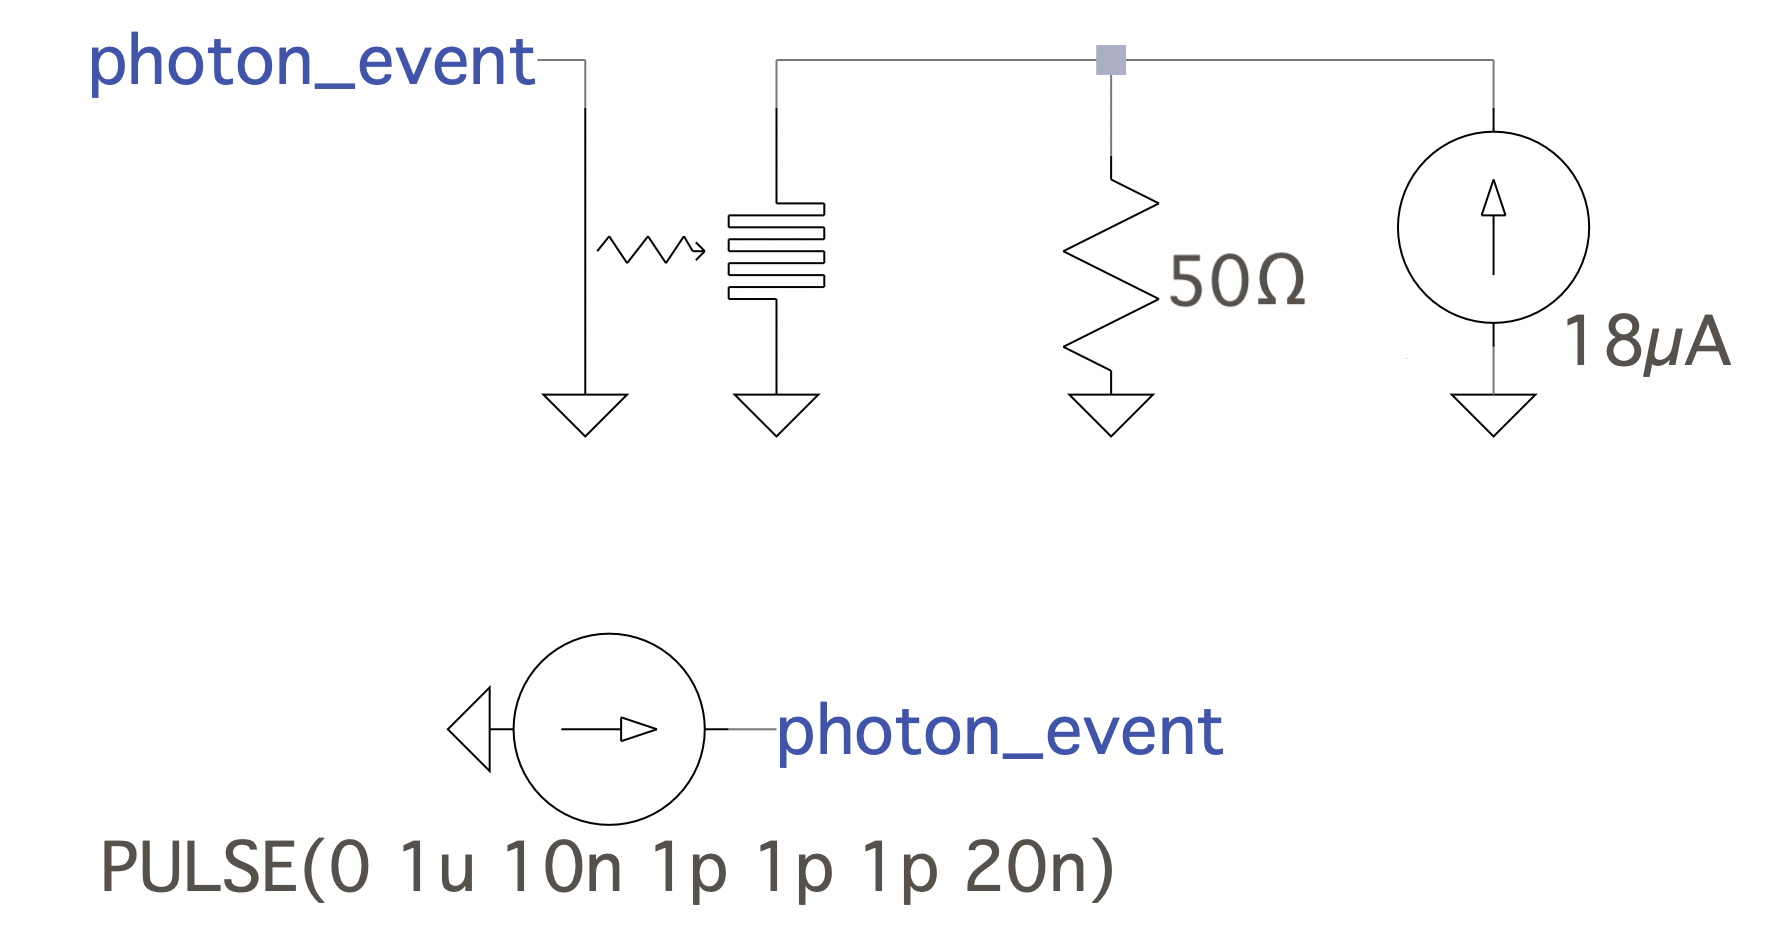
\includegraphics[width=0.4\textwidth]{figs/typical_circuit.png}}
    \subfigure[]{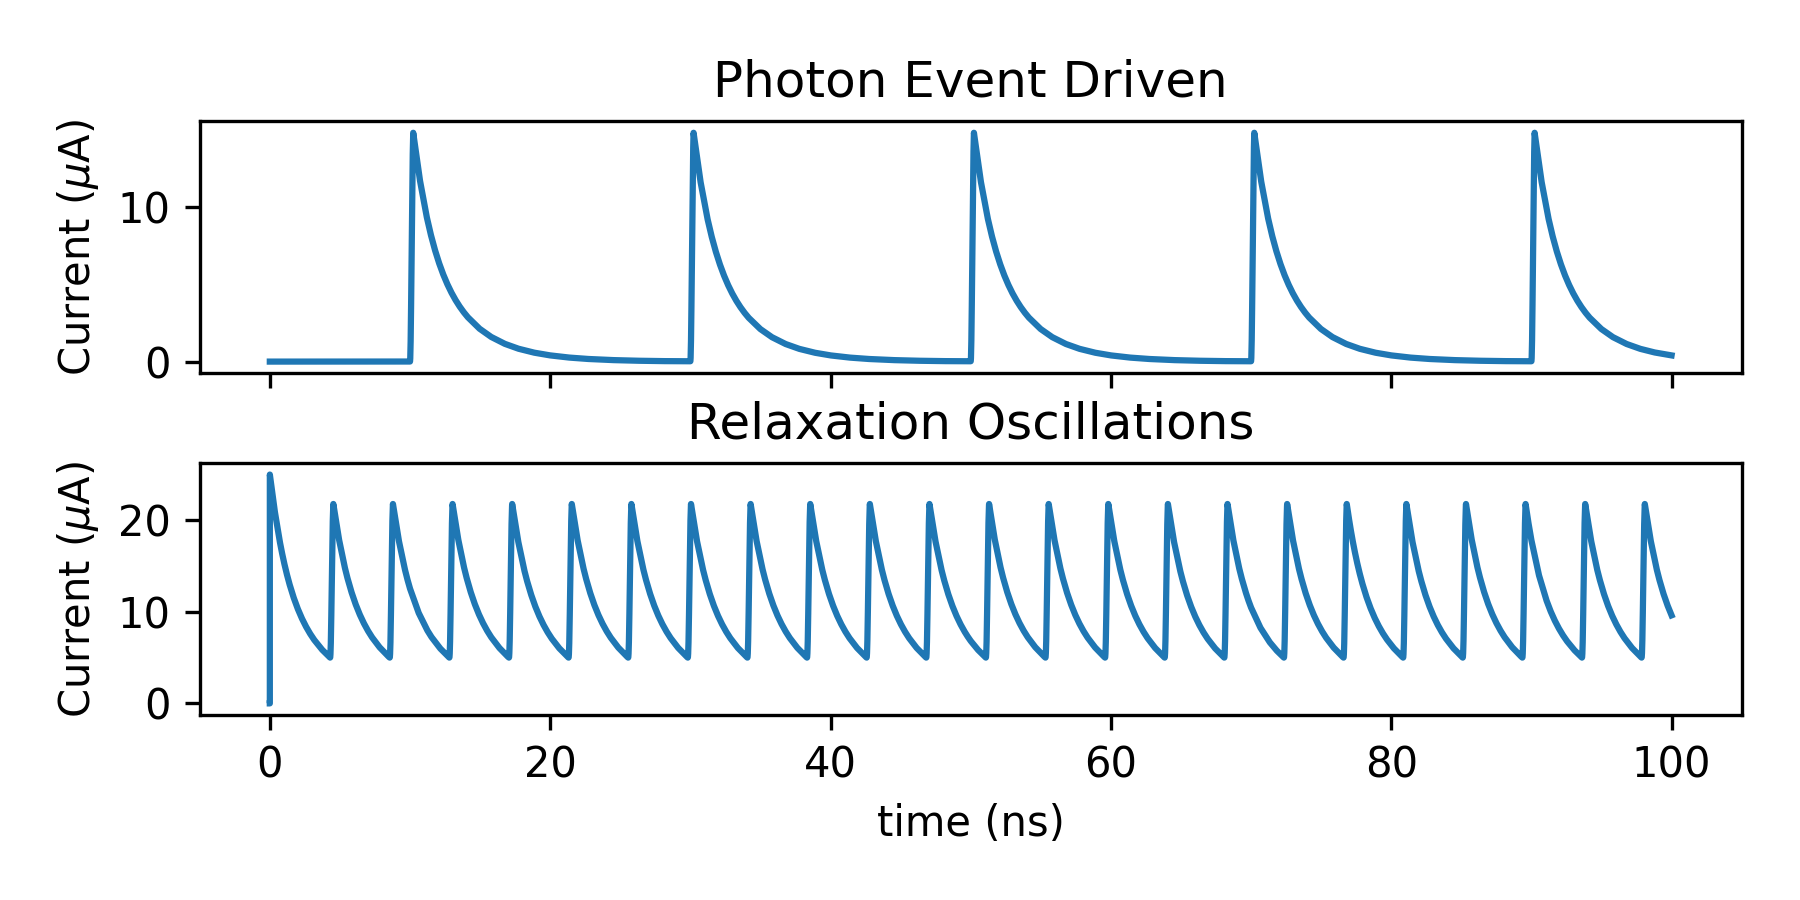
\includegraphics[width=0.58\textwidth]{figs/typical_snspd_out.png}}
    \caption{(a) Typical SNSPD readout circuit with a \qty{50}{\ohm} shunt resistor. (b)
    Two operation regimes for a nanowire with $i_c=\qty{21}{\micro\ampere}$ are shown. The top plot 
    is 5 separate photon detection events using a bias of \qty{18}{\micro\ampere}. The bottom plot
    showcases relaxation oscillation done by biasing the nanowire with \qty{25}{\micro\ampere}.}
    \label{fig:typical}
\end{figure}

In this topology, the nanowire can produce high frequency relaxation
oscillations when biased above the critical current \cite{relaxation_oscillations}.
These oscillations are caused by the
current periodically being diverted into and out of the resistive shunt. 
These relaxation oscillations consist of periodically repeating SNSPD spikes, 
similar to a switching event.

\subsection{SNSPIs} \label{snspi_intro}

Superconducting nanowire single-photon imagers (SNSPIs) are used in a similar fashion
to SNSPDs but take advantage of the distributed picture for longer nanowire meanders
 \cite{snspi_paper}.
SNSPIs tend to be designed to have a slower propagation velocity and longer meanders.
These effects cause a switching effect in the wire to take time to propagate to the two 
ends of the nanowire. By performing differential readout, we can spatially resolve
the photon's incidence location as a function of the delay between the 2 device ports.

\begin{figure}
    \centering
    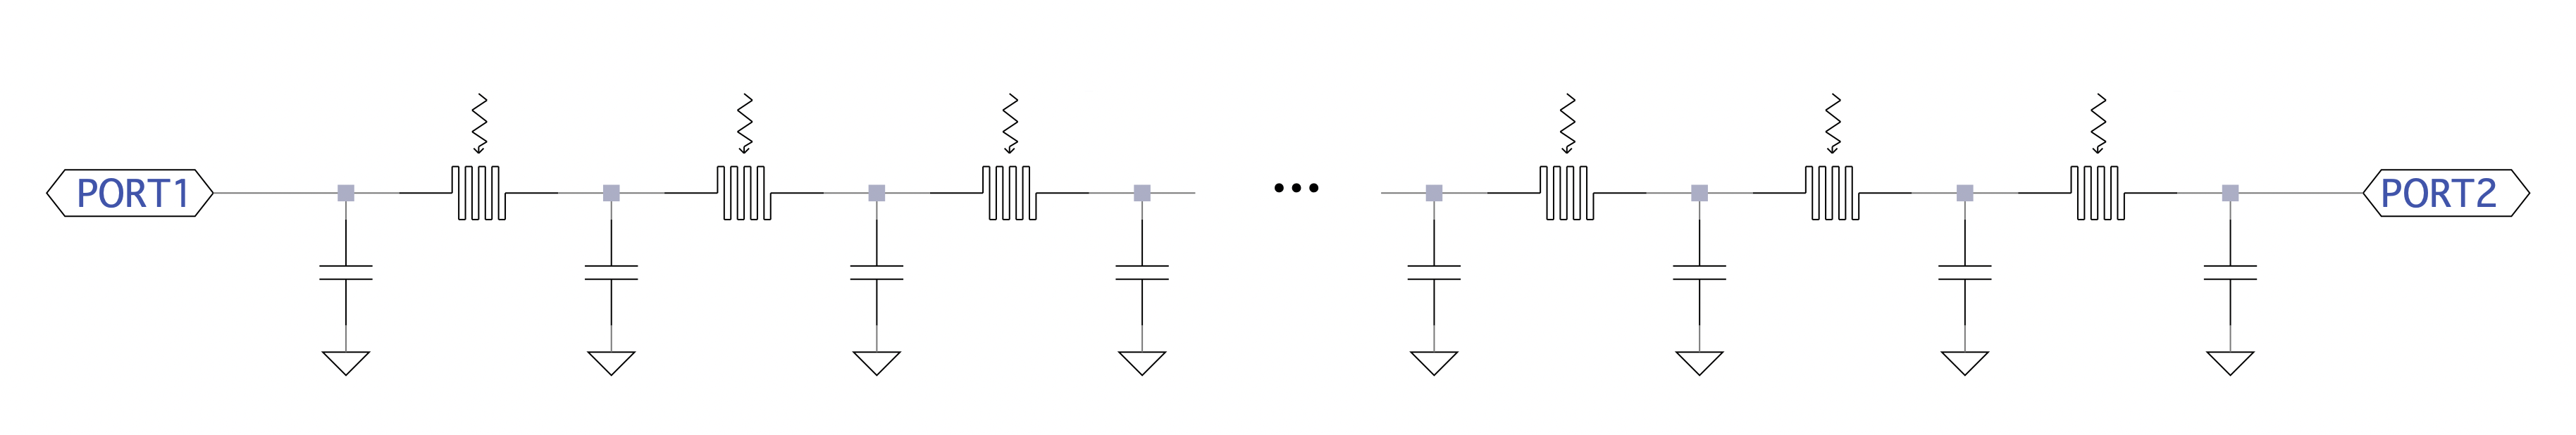
\includegraphics[width=\textwidth]{figs/snspi_meander.png}
    \caption{A lumped model approximation of an SNSPI meander. The model uses the same
    topology used to approximate distributed effects in linear transmission lines,
    swapping out the linear inductor with a non-linear nanowire.}
    \label{fig:snspi_tline}
\end{figure}
\todofig[]{SNSPI TLINE}

In this image, the SNSPI can be thought of as a non-linear transmission line that
has the additional state nonlinearities described in section \ref{nonlinearity}. By discretizing the transmission line
into multiple lumped elements, the local non-linear contributions can be modeled by a
non-linear inductor and resistor and a linear capacitor. In the distributed picture image,
a nanowire can be thought of as a long chain of discrete lumped nanowire elements in parallel
with linear capacitor elements as shown in figure \ref{fig:snspi_tline}. This topology captures the distributed picture of
pulses propagating in nanowire meanders and allows us to simulate SNSPIs.

\subsection{Impedance Matching Tapers} \label{tapers_intro}

Usually, the nanowire's impedance is not similar enough to that of the input and output circuitry. This mismatch causes the signal to reflect back into the wire instead 
of propagating into the next stage, causing interference and distortions. Impedance 
matching is done by designing tapers: extensions of the same line that increase in 
width slowly as shown in figure \ref{fig:thewiredesign}. This slow increase ensures 
that there is a minimal step change in impedance allowing for fewer overall reflections. A Klopfenstein taper is the optimal taper geometry when minimizing the total amount 
of reflections and the taper's length \cite{klopfenstein_transmission_1956}. 
The slow change in width still causes internal reflections along the length of the 
wire, however, their overall magnitude is smaller than one step change as illustrated in 
figure \ref{fig:whatsataper}.
\todoidea[inline]{mayhaps exponential taper, etc.}

Impedance matching tapers are often used on nanowire devices when we care about preserving
the signal shape and magnitude. Thus, tapers allow us to reduce jitter in SNSPDs and preserve logic pulses in
nanowire-based electronics \cite{snspd-tapers-paper, maximizing_ic_w_taper}. 
Impedance matching tapers can also be used to resolve the 
number of photons incident on an SNSPD \cite{pnr}.
Tapers are also used in SNSPIs, where the tapers
preserve the fast-rising edge that is essential for spatially
resolving photons \cite{snspi_paper}. 

\begin{figure}[h]
    \centering
  % \subfigure[]{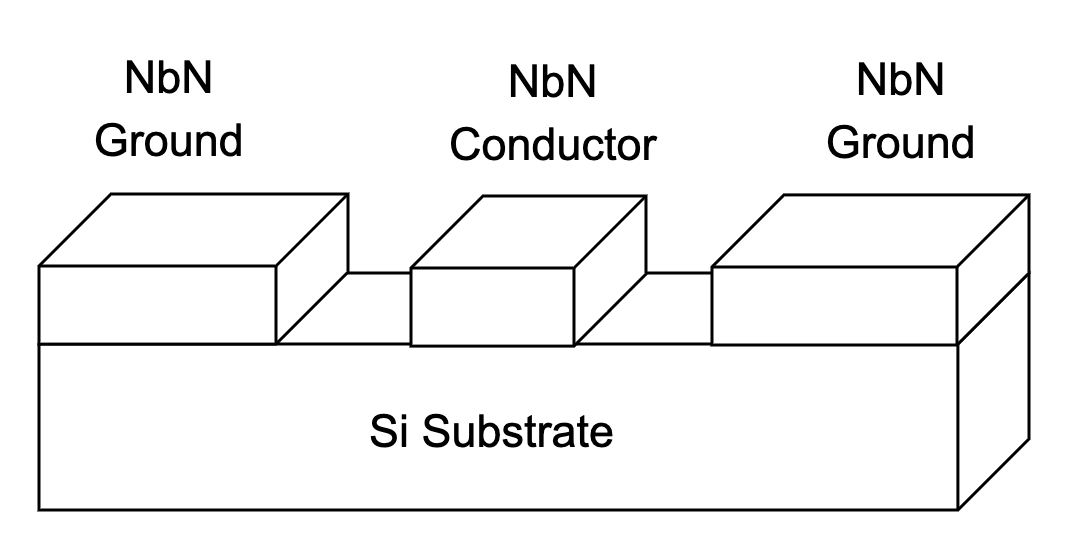
\includegraphics[width=0.35\textwidth]{figs/layers.png}\label{fig:cpwlayers}}
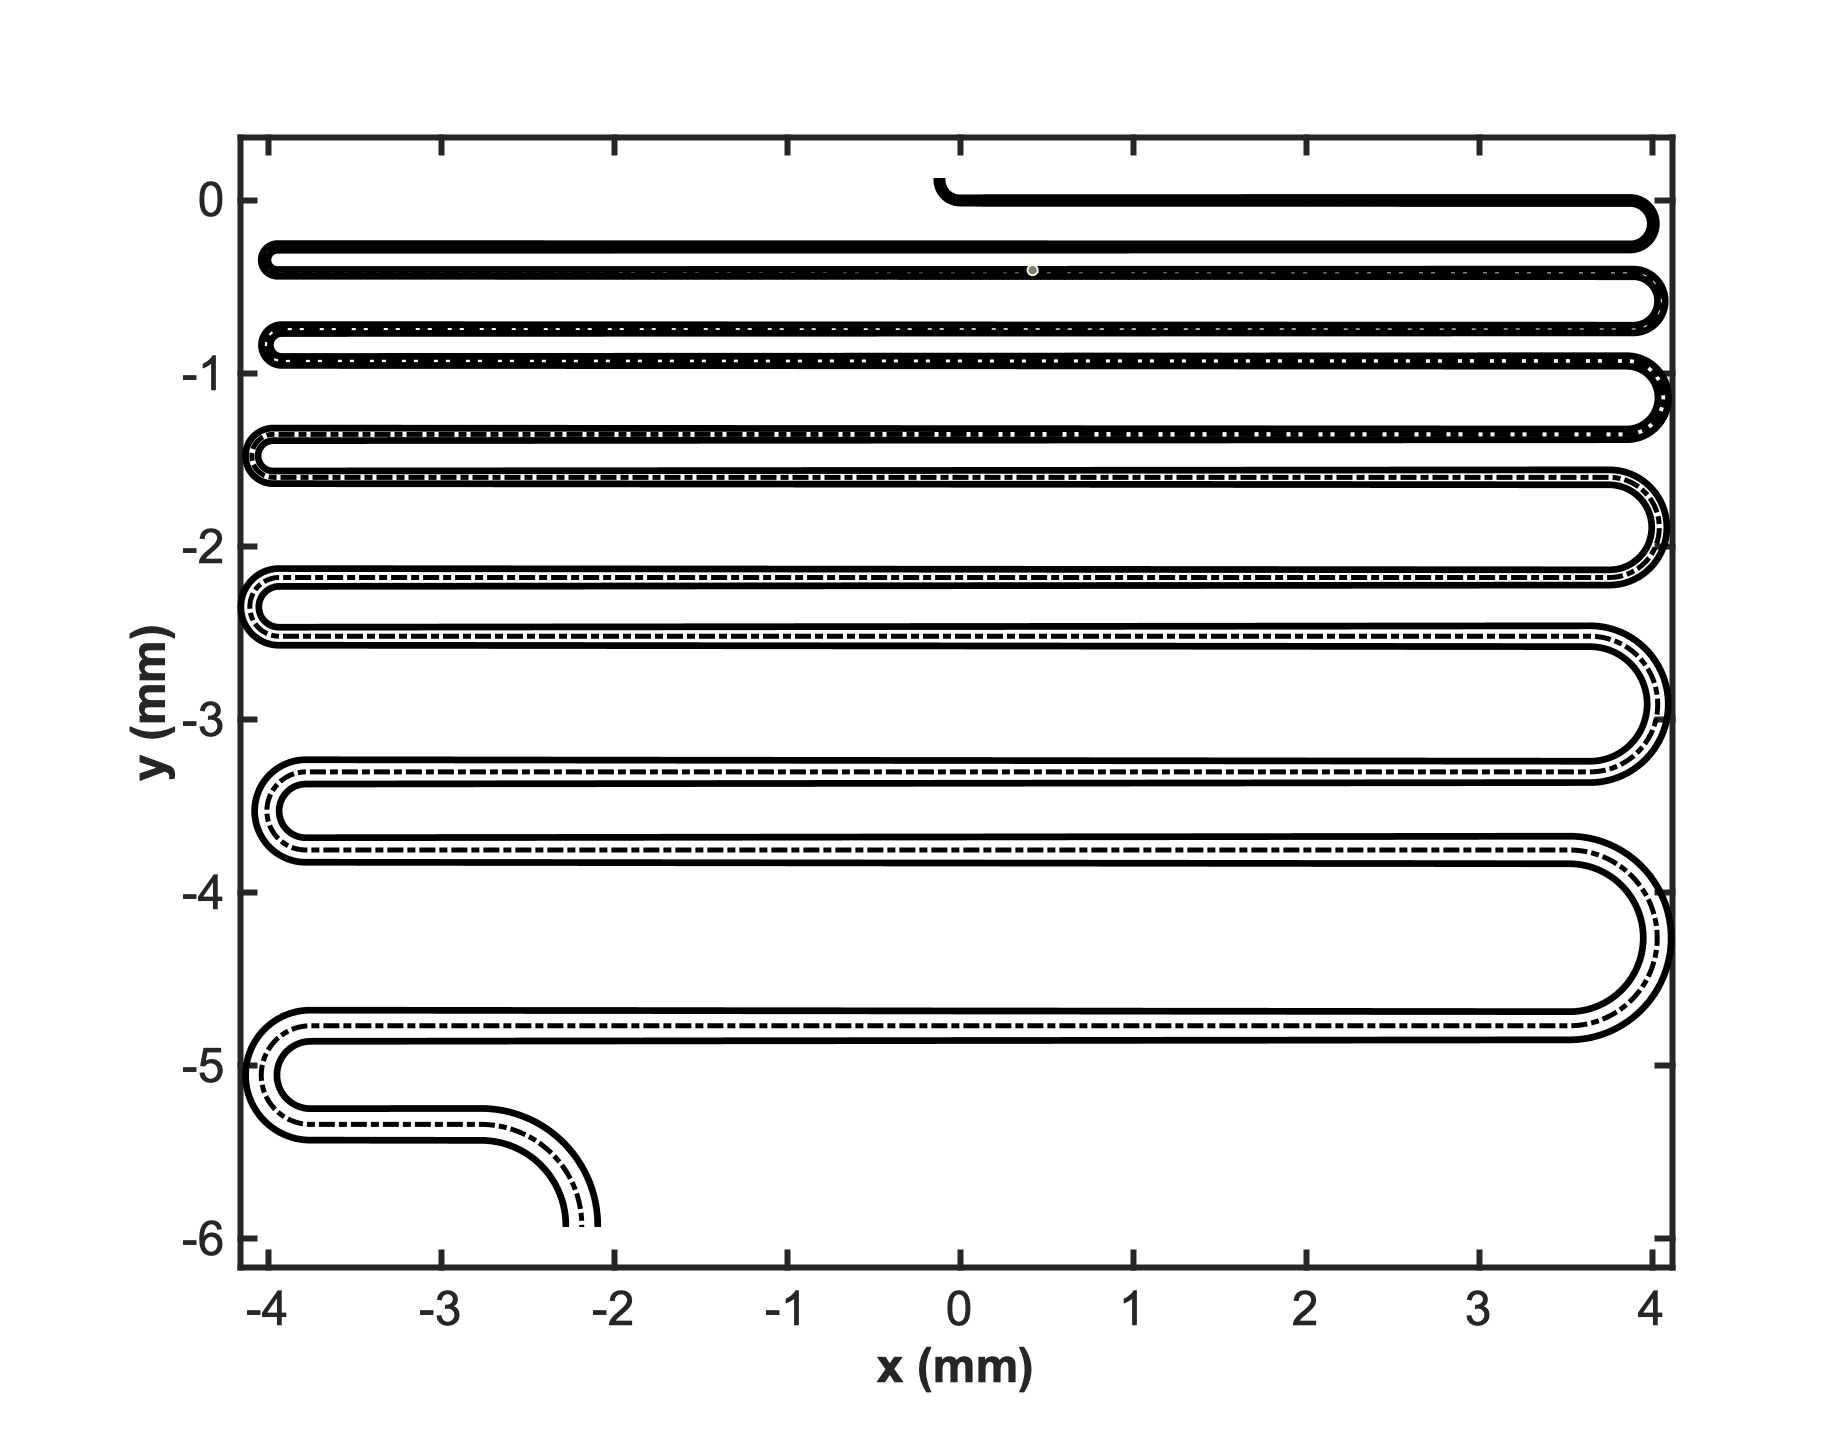
\includegraphics[width=0.5\textwidth]{figs/wire_matlab.png}
    \caption{Top view of a Klopfenstein taper with a folded meander.}
    \label{fig:thewiredesign}
\end{figure}

\begin{figure*}[h]
  \centering
  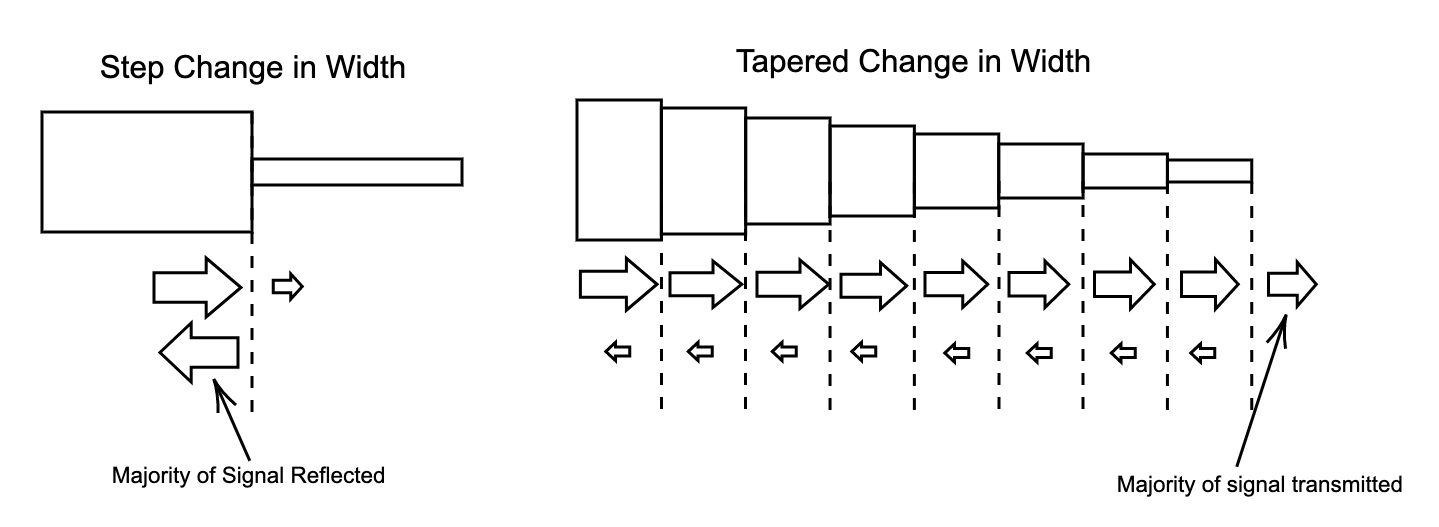
\includegraphics[width=5in]{figs/whatsataper.png}
  
  \caption{A tapered change in width causes smaller reflections at each boundary which add up to a lower total amount of reflection than a singular step change in width. Change in width is roughly proportional to change in impedance. The inclusion of multiple step changes in
  width increases the number of individual reflections occurring. 
  The number of interferences a simulator would need to keep track of grows 
  exponentially, increasing the complexity of the simulation.}
 \label{fig:whatsataper}
\end{figure*}

One side effect of using a Klopfenstein taper is the change in propagation velocity 
caused by the change of electrical characteristics in the wire. Using $L(x)$ and $C(x)$ 
as the inductance and capacitance along the length of the wire, 
the propagation velocity is dependent on $L\cdot C$ and varies along $x$ (since 
$L$ and $C$ do not scale inversely). Coupling this with the fact that the thinner wire will 
have a higher current density, this becomes a huge source of distortion.

Long tapers (and nanowires) are wound up in a 
boustrophedonic pattern of parallel straight wires 
connected by curved edges with 
large radii as shown in figure \ref{fig:thewiredesign}. This curvature is chosen in a manner that minimizes the total amount of reflection
and current crowding: an unwanted effect caused by non-homogeneous distributions 
of current density through a conductor that changes the frequency response and impedance 
of the wire \cite{Akhlaghi:12}. Impedance matching and the folding of 
the wire are both sources of distortions
to signals travelling down the meander. As a result accurate simulation requires the ability to account for both the taper reshaping and the coupling of the folds.

\subsection{hTron}

A nanowire's accessible state space is limited by its current thermal state.
Since the nanowire is also a thermal system that can generate heat,
modeling its thermal behavior is important for
accurate device characterization to account for effects such as latching 
\cite{electro_thermal_modelling}.

While this coupling can be unwanted, devices, such as the heater-tron (hTron), 
take advantage of that coupling \cite{htron_paper}. 
The hTron involves two superconducting stacks separated
by an insulating layer. One of the stacks contains a resistor that generates heat while the
other stack contains a nanowire above the resistor. When current flows through the resistor
it generates heat that gets transmitted through the stack to the nanowire. Through this thermal
coupling, the nanowire can be thermally biased.

Heat transport through the stack can be modeled as interactions between electrons 
and phonons \cite{htron_paper}. Each layer in the stack has
electron and phonon systems that can interact with other
layers at the boundaries.
The electron systems can be heated by Joule dissipation.
This model can account for heat generation, conduction
and dissipation.

\todo[]{reuse rezas thermal transport block diagram? and ref+cite it}

\section{Problems Simulating Nanowires}

A full-model that simulates all the dynamics of superconducting nanowires is hard to achieve
due to the complexity, long simulation time and convergence issues
that arise.
Previous parts of this section demonstrated multiple regimes nanowires can be used in,
from thermal coupling to a distributed microwave picture, each of which involves solving
stiff non-linear differential equations in the time domain. Getting a model to simulate
the electro-thermal coupling of a nanowire with respect to the stack, noise and photons
as well as the distributed effect accounting for nonlinearities results in stiff non-linear
equations. 
As a result of this complexity, work is usually done on the individual parts
with experimental fits for each picture but no model incorporating how these
different pictures interact. 

Berggren et al. implemented a nanowire model in LTspice based on the phenomenological hotspot 
velocity model developed by Kerman et al. \cite{karl_spice, phen_model}. 
This model is a lumped-element nanowire model that accounts 
for the hotspot dynamics using experimentally fitted parameters. It is implemented in LTspice
and contains both non-linearities exhibited by a nanowire -- discussed in more depth 
in section \ref{stability} \cite{karl_spice}. This model only 
accounts for the small-signal solution and cannot be used in noise, AC or DC analysis.
The model also suffers from instability around the state non-linearity to be discussed in section \ref{current_nw}. The instability and 
simulation modes are further discussed in section \ref{current_nw}.

Since the speed of the taper is not constant and the inductance is non-linear,
we expect input pulses to be reshaped non-trivially\todoidkcite{reshaping?}. Pulses traveling
in a taper experience reshaping due to the linear-taper aspect, the change in impedance
reflects certain components from the pulse while leaving other frequencies untouched.
When on its own, this reshaping can be completely captured by the scattering parameters and linear 
transmission lines. 
However,
non-linear transmission lines of constant width are also known to cause pulse reshaping, 
implying that scattering parameters on their own cannot fully describe a nanowire geometry
\cite{nl_tline_reshape}. 
Modeling tapers in LTspice tends to use a
sequence of transmission lines (namely the lossy transmission line model with $R=0$, 
discussed in \ref{tapers_section}) in series that have decreasing impedance. 
This model
is sufficient in simulating the linear part of the reshaping under the assumption
that the current flowing in the taper is much lower than the critical current, or
that in the DC picture, this effect reaches equilibrium and causes a final shift in the
perceived critical current of the device. In reality, this is not accurate, as pulses
being carried down a biased line also experience non-linear reshaping, which cannot
be accounted for by the linear transmission line segments.

Non-linear simulation for superconducting electronics has been widely studied in the 
frequency domain
using techniques like Harmonic Balance \cite{hb-book}. 
These methods can account for the continuous 
non-linearity presented by kinetic inductance, but not the state transition non-linearity.
These methods can generate scattering parameters that are dependent on frequency and
magnitude to account for the non-linearity.
JosephsonCircuits.jl for instance is designed
to simulate Josephson Traveling Wave Parametric Amplifiers (JTWPA) topologies in the frequency 
domain using Harmonic Balance \cite{josephsoncircsjl}. WRspice
and Xyce both have Harmonic Balance backends that are very efficient \cite{wrspice, xyce_reference}. However,
for topologies that utilize the binary-state non-linearity, time-domain simulation 
is needed to characterize the device behavior. Given the nature of WRspice and Xyce,
this constraint implies that the entire circuit must be simulated in the time-domain. This problem is
addressed in section \ref{julia-sim-hb}.

The non-linearity of the electrical model gets even harder to simulate when coupled to
a thermal equation. As a result, the thermal coupling is usually linearized around the 
regime we care about. For example, for nanowires that have no need to thermally
interact with other elements, the hotspot growth is simulated via the phenomenological
hotspot velocity model \cite{phen_model, matteo_thesis}. 
For geometries that rely on thermal coupling such as the hTron, the critical current
of the device is presumed to be a function of the electron temperature \cite{matteo_thesis}.
These models are sufficient for some applications but lack the ability to simulate the thermal behavior of the device,
neglecting the thermal coupling that might occur between two nanowires.
\todoidea[]{think about this more idk...}

While most of these effects are hard to simulate on their own, the simulation of multiple nanowires
is essential for scaling devices. As a result, it is important to develop 
a more stable scalable nanowire model, a dedicated efficient simulator, and a more standardized 
simulation environment that optimizes various nanowire topologies.

This thesis presents an integrated simulator environment designed with the goal of simulating
superconducting nanowires. Superconducting device
models have been designed to work in existing simulators
but tend to favor the frequency domain and can  
only account for 
the electrical non-linearities exhibited by superconductors \cite{josephsoncircsjl, wrspice}. 
Fast parallel circuit simulators with time and frequency domain capabilities
exist, such as Xyce from Sandia National Laboratories, are not optimized
for simulating superconducting nanowire geometries \cite{xyce_reference}.
The work presented in this thesis will be divided into 3 sections tackling: 
\begin{enumerate}
    \item an integrated environment for LTspice to design specific models and tools for superconducting 
    devices and accompanying experiments;
    \item a simple procedure to measure the stability of nanowire models used to 
    present an improved nanowire model; and
    \item finally, present preliminary work done to develop an efficient Julia-based simulator
    optimized for superconducting nanowire devices.
\end{enumerate}


\todoref[]{Latching: https://studylib.net/doc/11681854/electrothermal-feedback-in-superconducting-nanowire-singl...}

\todoref[]{Check this out: https://ieeexplore.ieee.org/document/4277823/figures#figures}

%%%%